\documentclass{article}

% If you're new to LaTeX, here's some short tutorials:
% https://www.overleaf.com/learn/latex/Learn_LaTeX_in_30_minutes
% https://en.wikibooks.org/wiki/LaTeX/Basics

% Formatting
\usepackage[utf8]{inputenc}
\usepackage[margin=1in]{geometry}

% Math
% https://www.overleaf.com/learn/latex/Mathematical_expressions
% https://en.wikibooks.org/wiki/LaTeX/Mathematics
\usepackage{amsmath,amsfonts,amssymb,mathtools}

% Images
% https://www.overleaf.com/learn/latex/Inserting_Images
% https://en.wikibooks.org/wiki/LaTeX/Floats,_Figures_and_Captions
\usepackage{graphicx,float}

% Tables
% https://www.overleaf.com/learn/latex/Tables
% https://en.wikibooks.org/wiki/LaTeX/Tables

% Algorithms
% https://www.overleaf.com/learn/latex/algorithms
% https://en.wikibooks.org/wiki/LaTeX/Algorithms
\usepackage[ruled,vlined]{algorithm2e}
\usepackage{algorithmic}

% Code syntax highlighting
% https://www.overleaf.com/learn/latex/Code_Highlighting_with_minted
\usepackage{minted}
\usemintedstyle{borland}


\usepackage{tikz}
\usetikzlibrary{positioning}

% Title content
\title{CS264A Homework 2}
\author{Bobby Judd}
\date{November 4th, 2020}

\begin{document}

\maketitle

% 1
\clearpage
\section{}
\begin{enumerate}
    \item $\{X, Y\},$
    \item $\{X, Z\},$
    \item $\{\lnot Y, W\},$
    \item $\{\lnot Z, \lnot W\},$
    \item $\{X, \lnot Y\},$
    \item $\{\lnot X, W\},$
    \item $\{\lnot X, \lnot W, V\},$
    \item $\{\lnot X, \lnot W, \lnot V\},$
    \item $\{Z, \lnot X\},$
    \item $\{\lnot Z, W\},$
    \newline
    \noindent\rule{4cm}{0.4pt}
    \item $\{Z\}$ \quad from 2 and 9
    \item $\{-Z\}$ \quad from 4 and 10
    \item $\{\}$ \quad from 11 and 12
\end{enumerate}
The minimal unsatisfiable core would be clauses 2, 4, 9, 10 or:
\[\{\{X, Z\}, \{\lnot Z, \lnot W\}, \{Z, \lnot X\}, \{\lnot Z, W\}\}\]

% 2 
\clearpage
\section{}
\renewcommand{\labelenumi}{(\alph{enumi})}
 \begin{enumerate}
   \item \[\Delta = (\lnot X), (X \lor Y), (X \lor Z), (\lnot Y \lor \lnot Z)\] \\
       \begin{center}
           \begin{tabular}{ |c|c|c|c| }
            \hline
             X&Y&Z&Cost \\ 
             \hline
             0&0&0&2 \\
             0&0&1&1 \\
             0&1&0&1 \\
             0&1&1&1 \\
             1&0&0&1 \\
             1&0&1&1 \\
             1&1&0&1 \\
             1&1&1&2 \\
             \hline
            \end{tabular} \\
            The optimal solution is a cost of 1
        \end{center}

   \item \[\]\\
    \begin{tikzpicture}[align=center]
    \node at (3,3) (x){$(X)$ \\ $(Z \lor \lnot X)$}[grow'=up, sibling distance=10em]
        child {
          node {$(\lnot Z)$ \\ $(Y \lor Z)$} 
            child {node {$(\lnot X \lor \lnot Y)$ \\ $(Y)$}
                  child {node (not_x) {$(\lnot X)$}edge from parent[<-]}
                  child {node {$(X \lor Y)$} edge from parent[<-]}
                  edge from parent[<-]
                }
            child {
                node {$(\lnot Y \lor \lnot Z)$} edge from parent[<-]}
                edge from parent[<-]
        }
        child{
            node {$(X \lor Z)$}
            edge from parent[<-]
        };
        
    \node[draw] at (0, 0) (x_false) {false};
    \draw [->] (x) -- (x_false);
    \draw [->] (not_x) -- (x_false);
    \end{tikzpicture}
 \end{enumerate}

% 3
\clearpage
\section{}
\[\Delta = (A \lor B \lor C), (\lnot A \lor D \lor E)\]
\begin{center}
    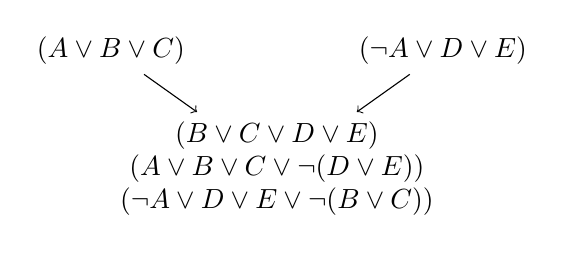
\begin{tikzpicture}[align=center]
        \node {$(B \lor C \lor D \lor E)$ \\
                $(A \lor B \lor C \lor \lnot (D \lor E))$ \\
                $(\lnot A \lor D \lor E \lor \lnot (B \lor C))$}[grow'=up, sibling distance=12em]
          child {node {$(A \lor B \lor C)$}edge from parent[<-]}
          child {node {$(\lnot A \lor D \lor E)$} edge from parent[<-]};
    \end{tikzpicture}
\end{center}

 % 4
 \clearpage
 \section{}
 \begin{enumerate}
     \item Enumerate possibilities of $\Delta = (\lnot D \lor \lnot E \lor B),(\lnot B \lor E \lor \lnot A),(\lnot D \lor C \lor \lnot B),(\lnot B \lor C \lor E)$:
     \begin{center}
           \begin{tabular}{ |c|c|c|c|c|c| }
            \hline
             A&B&C&D&E&Output \\ 
             \hline
             T&T&T&T&T&True \\
            T&T&T&T&F&False \\
            T&T&T&F&T&True \\
            T&T&T&F&F&False \\
            \hline
            T&T&F&T&T&False \\
            T&T&F&T&F&False \\
            T&T&F&F&T&True \\
            T&T&F&F&F&False \\
            \hline
            T&F&T&T&T&False \\
            T&F&T&T&F&True \\
            T&F&T&F&T&True \\
            T&F&T&F&F&True \\
            \hline
            T&F&F&T&T&False \\
            T&F&F&T&F&True \\
            T&F&F&F&T&True \\
            T&F&F&F&F&True \\
            \hline
            F&T&T&T&T&True \\
            F&T&T&T&F&True \\
            F&T&T&F&T&True \\
            F&T&T&F&F&True \\
            \hline
            F&T&F&T&T&False \\
            F&T&F&T&F&False \\
            F&T&F&F&T&True \\
            F&T&F&F&F&False \\
            \hline
            F&F&T&T&T&False \\
            F&F&T&T&F&True \\
            F&F&T&F&T&True \\
            F&F&T&F&F&True \\
            \hline
            F&F&F&T&T&False \\
            F&F&F&T&F&True \\
            F&F&F&F&T&True \\
            F&F&F&F&F&True \\
             \hline
            \end{tabular} \\
        \end{center}
        There are 20 variable instantiations that satisfy $\Delta$ and 12 that do not. Yes, the majority of variable instantiations satisfy this KB.
        \item The solution to E-MAJ-SAT is Yes.  An example instantiation that  shows this is:
        \begin{center}
           \begin{tabular}{ |c|c|c|c|c|c| }
                \hline
                 A&B&C&D&E&Output \\ 
                 \hline
                T&F&T&T&T&False \\
                T&F&T&T&F&True \\
                T&F&T&F&T&True \\
                T&F&T&F&F&True \\
                 \hline
                \end{tabular} \\
        \end{center}
        For the variable instantiation for: $X = (A=t, B=f, C=t)$ 3 out of 4 settings for $Y = (D,E)$ are true, which is a majority.
        
        \item Similar to part (b), we will use a given (A,B,C) instantiation to determine if the majority of (D,E) instantiations have a majority of True. Referencing the table in part (a) you can see for the 8 different instantiations of X, 5 of the corresponding Y's result in a majority of True, and 3 do not.  Which confirms MAJ-MAJ-SAT for $X=\{A,B,C\}$ and $Y=\{D,E\}$
 \end{enumerate}
 % 5
 \clearpage
 \section{}
 \[ \Delta = \begin{cases} 
      A \iff P_{A} \\
      \lnot A \iff P_{\lnot A} \\
      A \lor B \iff P_{B|A} \\
      \lnot A \lor B \iff P_{B|\lnot A} \\
      A \lor \lnot B \iff P_{\lnot B|A} \\
      \lnot A \lor \lnot B \iff P_{\lnot B|\lnot A} \\
      B \lor C \iff P_{C|B} \\
      \lnot B \lor C \iff P_{C|\lnot B} \\
      B \lor \lnot C \iff P_{\lnot C|B} \\
      \lnot B \lor \lnot C \iff P_{\lnot C|\lnot B}
   \end{cases}
\]
The weighted models that are consistent with A=T C=F are:
\[\theta_{A}\theta_{B|A}\theta_{\lnot C|B} = (0.6)(0.8)(0.75) = 0.36\]
\[\theta_{A}\theta_{\lnot B|A}\theta_{\lnot C|\lnot B} = (0.6)(0.2)(0.7) = 0.21\]

The margin probability of A=T and C=F would be the sum of the two model weights: \textbf{0.57}
 % 6
 \clearpage
 \section{}
The NNF circuit is not decomposable following reasons:
\begin{itemize}
    \item $and^{3}$ contains C in the left and right branches
\end{itemize}
The NNF circuit is not deterministic following reasons:
\begin{itemize}
 \item $or^{4}$ is not mutually exclusive, A and B could both be True.
 \item $or^{5}$ is not mutually exclusive, $\lnot C$ and $\lnot A$ could both be True.
 \item $or^{1}$ is not mutually exclusive. Which is shown if you enumerate possibilities for A, B, and C for this NNF.
\end{itemize}
 % 7
 \clearpage
 \section{}

% 8
\clearpage
\section{}

% 9
\clearpage
\section{}

% 10
\clearpage
\section{}

\end{document}